\problemname{Musical Mending}

Shortly before the concert starts, you notice that your piano is completely out
of tune! Having the ability of relative pitch, you are able to discern the
difference between the pitch of any piano key to the first piano key. While this
does not help you find the absolute pitch, you decide to at least tune the keys relative
to each other. To do this, you need to make sure that the pitch of each key is exactly one 
higher than the key before it and one lower than the key after it.
As the concert will start shortly, you need to minimize the total tuning effort,
which is the sum of the absolute changes in pitch you apply to each key.
For example, Figure~\ref{fig:piano} illustrates a solution for Sample Input 3, resulting in a total tuning effort of 23.

\begin{figure}[!h]
	\centering
	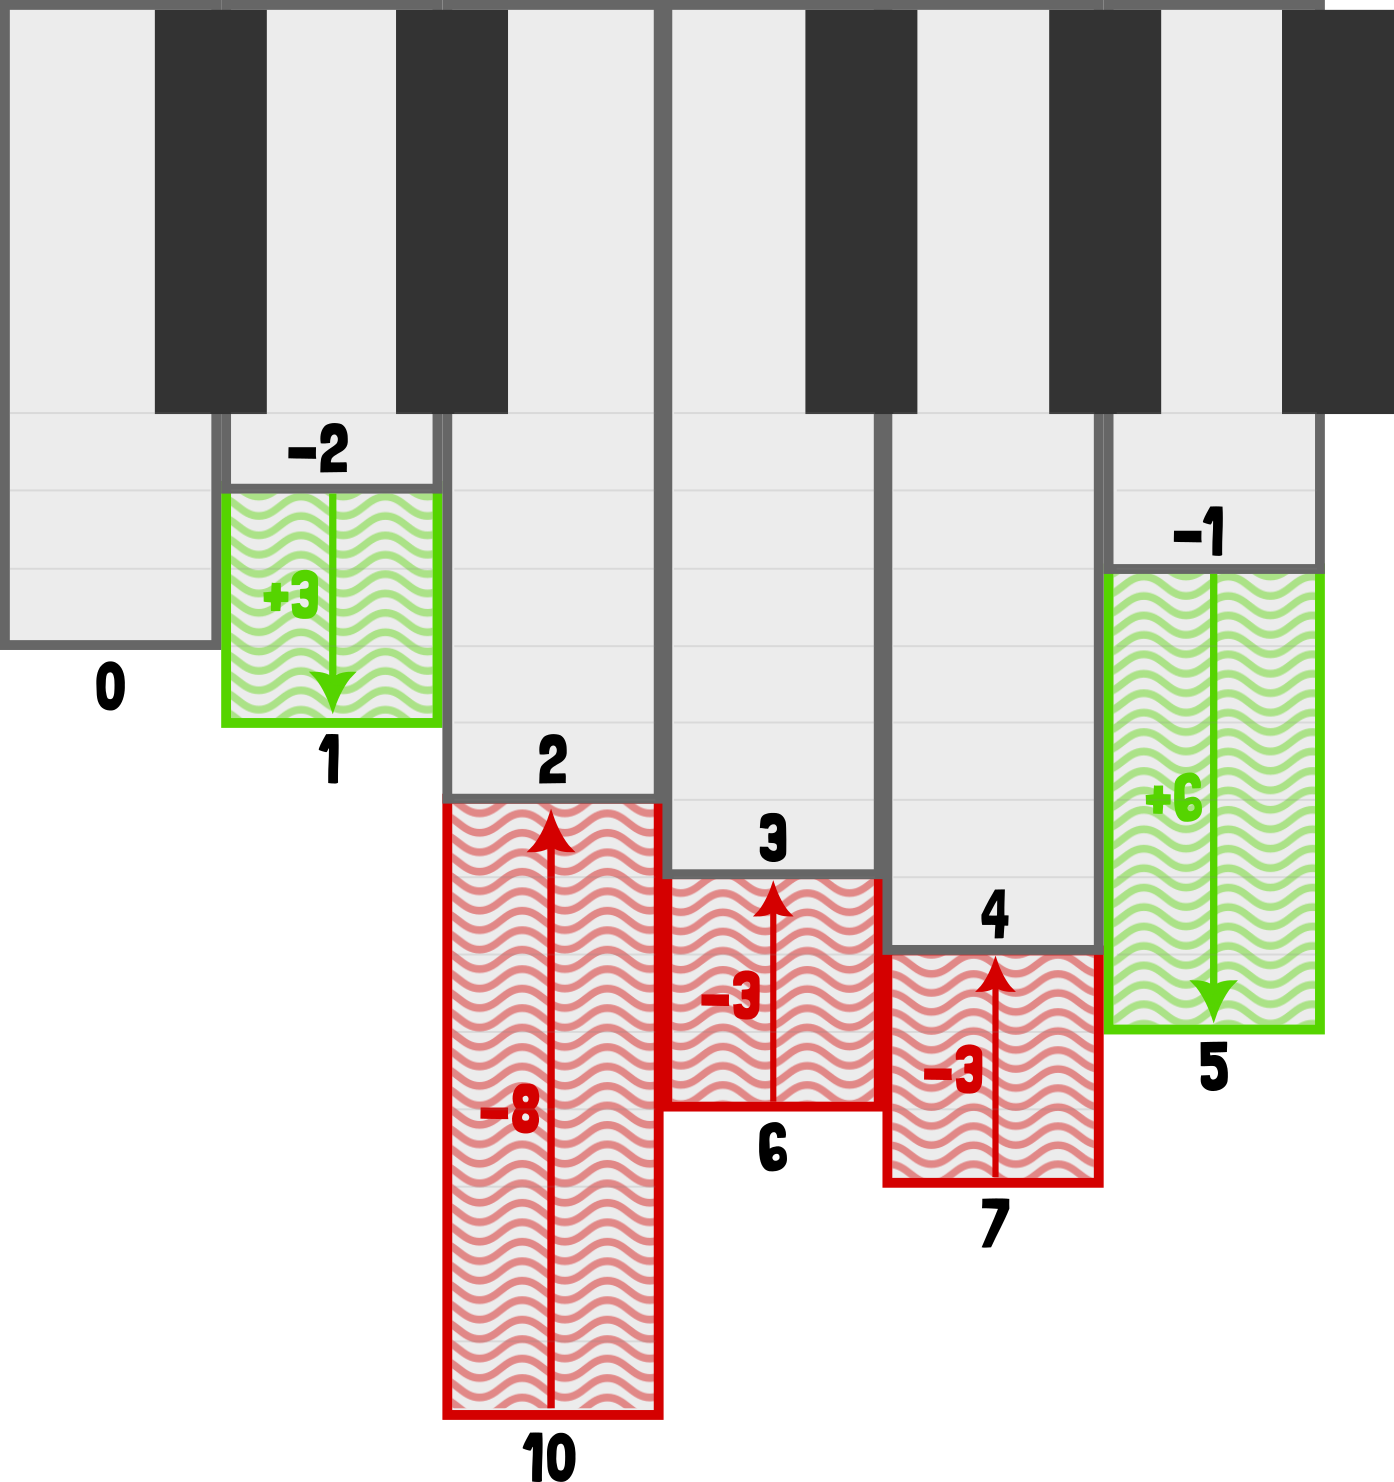
\includegraphics[width=0.4\textwidth]{sample3_v7.png}
	\caption{Visualization of Sample Input 3.}
	\label{fig:piano}
\end{figure}

\begin{Input}
  The input consists of:
  \begin{itemize}
    \item One line with an integer $n$ ($2 \leq n \leq 10^5$), the number of keys on the piano. 
    \item One line with $n$ integers $t_1,\dots,t_n$ ($-2 \cdot 10^5 \leq t_i \leq 2 \cdot 10^5$), where $t_i$ describes the difference in pitch between the $i$th key and the first key.     
      % omitting 'for each $i$' intentionally, despite the styleguide, as suggested by Michael
      The first integer $t_1$ is always $0$.    
  \end{itemize}
\end{Input}

\begin{Output}
  Output the minimal total tuning effort.
\end{Output}
